\chapter{Conclusion}

Goal of investigation of available numerical methods was accomplished, the topic is very deep with all of the subproblems: dynamic system modeling, transcription, algebraic modeling, mesh refinement, NLP solving, sparse linear solving, sensitivity analysis and frameworks that encompass them being infinitely deep I CAN SPEND INFITE TIME LEARNING THEM. It was difficult to understand these topics in meaning ful way without spend too much time on a single topic.  

More investigation would be nice into differentiate orthogonal polynomials, Chebyshev type I. polynomials are often used with high order due to their good suppression of Runge phenomena. 

As for NLP solvers a better set of options can be found for Ipopt by investigating why the solver fails in some cases, also it may make sense to try Uno solver~\cite{vanaret_implementing_2025} and construct a new specialized solver for this problem, but that would take enormous amount of time.

Building a model for optimization was difficult, as debugging it is difficult, when the grid is sampled too densely or different thins are not good, Ipopt fails to converge. I wasn't using any tool to find which constraint is causing this, debugging could be improved by writing/using a tool which would tell which constraint is causing issues. This would significantly decrease the development time.

h method implemeted is not good very bad better needs to be implementd the rror estimation is only placeholder TODO

As for implementation, Julia was interesting language to learn, it offers blazing fast execution, but that comes with caveats. Debugging is way more complicated. When working on a smaller project, the debugging is not such a pain, but when the project is bigger debugging is not user friendly. Debugging in python and MATLAB is way easier. Julia's main selling point is that it is just in time compiled language, rivalling C after compilation. That is true BUT you have to know what you are doing, if you don't, it can be as slow as python. Also JuMP was taking 90\% of NLP solving time on calculating the derivatives, when constraints had dense expressions~\cite{julia_discourse_ipopt_hessian,julia}, so only 10\% by the actual solver, CasADi seems not to have this issue also implementation using automatic differentiation from ExaModels~\cite{shin2024accelerating} on GPU would be beneficial to experiment with.TODO

One thing which was not a goal but, would be super useful if i managed to do a validation of sensitivity analysis on real world data. That is driving vehicle on track, measuring time, loading sand bags (and/or myself as passenger) as extra weight into the car and driving again. I wanted to do it for a long time but there was not enough of time. TODO

At the begging of this project I wanted a more complex model, I wanted to go deeper with complexity than my bachelor thesis. That is add pitch, roll and add suspension with damper and spring for each wheel, add Equivalent circuit model 1RC for the accumulator, properly implement energy accumulation, add road bank and inclination. Investigate the possible implementations of losses from Section~\ref{motormodel} and using softmax or different approximations. Also this simulation does not account for gearboxes with discrete stages, and no combustion engine.TOODO

Believing 100\% this tool and designing car according to it would most likely lead to undriveable vehicle, as objective of time minimization doesn't account for stability and driveability, \cite{perantoniOptimalControlFormula2014} deals also with this. The optimal driving created by NLP is unachievable by real driver, as the vehicle is on its limit and one mistake would overload tires and cause failure.TODO

the comparison is biased towards high number, the total time should not be relative to total time of all solver or timeof longest solve. Also median is not telling much with so few samples.
TODO

Automated behncmarking is a must becasue small canges can break many things and you may notice the simulation crashing long after iplementaton also objetive time should be evlauated in similar graph manner. QWERTA
QWERTA

implement softmax and max approximaitons




%\section{Conditions of optimality for constrainednoptimization}
%This chapeter derives conditions which given popint must satisfy if it is optimal, Algorithms for finding these points will be described in next chapter. My goal is to buid the theory in digestable way,for people not fluent in nonlinear optimisation I will start with simple example to explain main ideas clearly
%and then generalise it to create optimisation framework. Very good intuitive itroduction is given in this youtube video \cite{cite:48}
%Simplest useful example is: Find $x_1$ and $x_2$ that minimise the objective function $J(\mathbf{x}) = x_1^2+x_2^2$, subject to constraint function $c(\mathbf{x}) = x_1+x_2+3$. 
%\begin{mini}[2]
%{}{J(\mathbf{x})}{}{}
%\addConstraint{c(\mathbf{x})=0}
%\end{mini}
%with variables $x_1,x_2\in\mathbf{R}$. 
%This is visualised on contour plot of $J(\mathbf{x})$ Figure \ref{eq:constrained_optim}, orange line is constraint function, red arrow are vectors of gradient at each point. The solution must lie somewhere on the orange constraint line.
%From the figure it can be easily seen that the optimum is on the point where the constraint line 
%of $x_1+x_2+3 =0$ is tangent with contour circle of $x_1^2+x_2^2$.
%In other words, the constraint line is perpendicular to the gradient at the optimal point, this means that 
%gradient of $J(\mathbf{x})$ and gradiebnt of  $ c(\mathbf{x})$ differ only in their scale in the optimal point, to symbolize their difference in scale, scalar variable $\lambda$ is introduced.
%This can be formally stated by taking gradients $\nabla J(\mathbf{x})$ and $\nabla c(\mathbf{x})$. and writing equation
%erafad
%\begin{equation}
%\nabla J(\mathbf{x}) = \lambda \nabla c(\mathbf{x})\label{eq:lagrange}
%\end{equation}
%\begin{equation}
%\nabla (J(\mathbf{x}) + \lambda c(\mathbf{x}))= 0\label{eq:dlagrangen}
%\end{equation}
%
%\begin{figure}[!h]
%\centering
%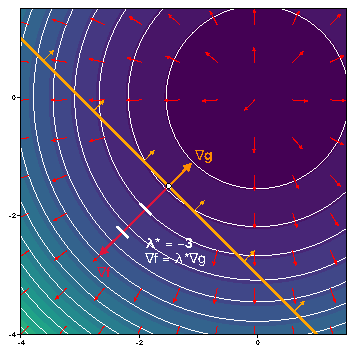
\includegraphics[width=0.8\textwidth]{../src/examples/constrained_optimum.pdf}
%\caption{Test}
%\label{eq:constrained_optim}
%\end{figure}
%
%By introducing more constraints to $c(\mathbf{x}) =0$, first order necessary conditions of optimality are stated%  \ref{eq:lagrange} 
%
%\begin{equation}
%\nabla J(\mathbf{x}) + \symbf{\lambda} \nabla c(\mathbf{x})= 0  \label{eq:first_order},
%\end{equation}
%\begin{equation}
%c(\mathbf{x})= 0.
%\end{equation}
%Point which satisfies this conditions is either optimum, minimum or saddle point
%$\lambda$ is  known as Lagrange multiplier,it is not some meaningless valuable that is be thrown away after finding the solution.  $\lambda$ can be thought of as a measure of importance of given constraint on the objective function $J(\mathbf{x})$,this concept is particularly useful for sensitivity analysis. Formally: $\lambda$ quantifies the sensitivity of the optimal cost to the constraint: $\frac{dJ^*}{d c(\mathbf{x})} = -\lambda$, where $\varepsilon$ is a small perturbation to $c(\mathbf{x}) = \varepsilon$. A large $|\lambda|$ means the constraint is strongly limiting the optimum, $\lambda = 0$ means the constraint is inactive and could be removed without affecting $J^*$, aaah i should make sure it is like this.
%
%
%\subsection{Inequality constrained optimization}
%
%Covered in section \ref{subsection:barrier_problem_formulation}.
%
%\chapter{Transcription}
%this chapter deal with the problem of transcribing the continuous optimal control problem into direct optimization problem, that is with discrete states and controls. The task boils down to integrating a function by evaluating it at discrete steps, this is called quadrature. The most commonly used quadratures for optimal control are Gauss-Legendre, Gauss-Radau and Gauss-Lobatto. Methods which are using these quadratures are called pseudospectral collocation methods. These methods are representing the integral of the function using polynomial, they are called collocation methods, because they work by forcing the derivation of the approximating polynomial to be equal to right hand side of the differential equation it is solving. Key aspect of these methods is that they can represent the solution to differential equation without error up to the degree of approximating polynomial. pridat toto s konstantou ktora big O little o...
%
%The approximating polynomials are constructing with roots of legendre, sometinh something lagrange polynomials
%DX = F(X,U)
%
%barycentric weights
%
%
%
%collocation point = derivation is equal to the differential equation
%boundary point = the constraints to tie two segment together are used for the solution
%
%gauss legendre points odnt contain any of the endpoint, the endpoints have to be constrained by extra addConstraint
%gauss legendre collocation
%N is in number of collocation points, order of approximating polynomial is then  for LG = 2N-1, for LGR = 2N-2, for LGL = 2N-3






%\part{My Party}
%
%
%\part{Your Party}
%
%\blindmathtrue
%
%\blinddocument
%
%\begin{table}
%\begin{ctucolortab}
%\begin{tabular}{cc}
%\bfseries Foo & \bfseries Bar \\\Midrule
%foo1 & bar1 \\
%foo2 & bar2
%\end{tabular}
%\end{ctucolortab}
%\caption{Foobar.}
%\label{tab:foobar}
%\end{table}
%
%\begin{figure}
%
\includegraphics[width=0.4\textwidth]{ctu_logo_black}
%\caption{Black logo of the CTU in Pragueueue.}
%\end{figure}
%
%\begin{figure}[!t]
%
\includegraphics[width=0.4\textwidth]{ctu_logo_blue}
%\caption{Blue logo of the CTU in Pragueueue.}
%\end{figure}   
%
%\chapter{Conclusions}
%
%\section{Test --- this is just a little test of something in the table of contents}
%
%\subsection{Yes, table of contents}
%
%\begin{theorem}\begin{enumerate} \item Bla \item Blo \end{enumerate} \end{theorem}
%
%
%Lorem ipsum dolor sit amet, consectetur adipiscing elit. Duis interdum facilisis urna, at tincidunt leo consectetur non. Maecenas bibendum mi vitae libero pharetra, ac ullamcorper nulla pellentesque. Sed sit amet massa nunc. Aenean placerat a est sodales sagittis. Quisque purus nibh, auctor ut consectetur at, suscipit non erat. Donec condimentum porttitor risus, vitae fringilla lectus tincidunt nec. Nulla leo quam, commodo eu ornare non, iaculis sed nulla. Duis gravida lacus quis purus sodales, vitae malesuada justo ultricies. Vestibulum nisl nulla, commodo non pellentesque a, fringilla a risus. Ut quis magna nulla. Mauris vitae ultricies ante, in consectetur justo. 
%
%\medskip
%
%\begin{proof}\begin{enumerate} \item[8] Bla \item Blo \end{enumerate} \end{proof}
